% Options for packages loaded elsewhere
\PassOptionsToPackage{unicode}{hyperref}
\PassOptionsToPackage{hyphens}{url}
%
\documentclass[
  ignorenonframetext,
]{beamer}
\usepackage{pgfpages}
\setbeamertemplate{caption}[numbered]
\setbeamertemplate{caption label separator}{: }
\setbeamercolor{caption name}{fg=normal text.fg}
\beamertemplatenavigationsymbolsempty
% Prevent slide breaks in the middle of a paragraph
\widowpenalties 1 10000
\raggedbottom
\setbeamertemplate{part page}{
  \centering
  \begin{beamercolorbox}[sep=16pt,center]{part title}
    \usebeamerfont{part title}\insertpart\par
  \end{beamercolorbox}
}
\setbeamertemplate{section page}{
  \centering
  \begin{beamercolorbox}[sep=12pt,center]{part title}
    \usebeamerfont{section title}\insertsection\par
  \end{beamercolorbox}
}
\setbeamertemplate{subsection page}{
  \centering
  \begin{beamercolorbox}[sep=8pt,center]{part title}
    \usebeamerfont{subsection title}\insertsubsection\par
  \end{beamercolorbox}
}
\AtBeginPart{
  \frame{\partpage}
}
\AtBeginSection{
  \ifbibliography
  \else
    \frame{\sectionpage}
  \fi
}
\AtBeginSubsection{
  \frame{\subsectionpage}
}

\usepackage{amsmath,amssymb}
\usepackage{iftex}
\ifPDFTeX
  \usepackage[T1]{fontenc}
  \usepackage[utf8]{inputenc}
  \usepackage{textcomp} % provide euro and other symbols
\else % if luatex or xetex
  \usepackage{unicode-math}
  \defaultfontfeatures{Scale=MatchLowercase}
  \defaultfontfeatures[\rmfamily]{Ligatures=TeX,Scale=1}
\fi
\usetheme[]{default}
\useinnertheme{circle}
\useoutertheme{default}
\usepackage[]{libertinus}
\ifPDFTeX\else  
    % xetex/luatex font selection
\fi
% Use upquote if available, for straight quotes in verbatim environments
\IfFileExists{upquote.sty}{\usepackage{upquote}}{}
\IfFileExists{microtype.sty}{% use microtype if available
  \usepackage[]{microtype}
  \UseMicrotypeSet[protrusion]{basicmath} % disable protrusion for tt fonts
}{}
\makeatletter
\@ifundefined{KOMAClassName}{% if non-KOMA class
  \IfFileExists{parskip.sty}{%
    \usepackage{parskip}
  }{% else
    \setlength{\parindent}{0pt}
    \setlength{\parskip}{6pt plus 2pt minus 1pt}}
}{% if KOMA class
  \KOMAoptions{parskip=half}}
\makeatother
\usepackage{xcolor}
\newif\ifbibliography
\setlength{\emergencystretch}{3em} % prevent overfull lines
\setcounter{secnumdepth}{-\maxdimen} % remove section numbering


\providecommand{\tightlist}{%
  \setlength{\itemsep}{0pt}\setlength{\parskip}{0pt}}\usepackage{longtable,booktabs,array}
\usepackage{calc} % for calculating minipage widths
\usepackage{caption}
% Make caption package work with longtable
\makeatletter
\def\fnum@table{\tablename~\thetable}
\makeatother
\usepackage{graphicx}
\makeatletter
\def\maxwidth{\ifdim\Gin@nat@width>\linewidth\linewidth\else\Gin@nat@width\fi}
\def\maxheight{\ifdim\Gin@nat@height>\textheight\textheight\else\Gin@nat@height\fi}
\makeatother
% Scale images if necessary, so that they will not overflow the page
% margins by default, and it is still possible to overwrite the defaults
% using explicit options in \includegraphics[width, height, ...]{}
\setkeys{Gin}{width=\maxwidth,height=\maxheight,keepaspectratio}
% Set default figure placement to htbp
\makeatletter
\def\fps@figure{htbp}
\makeatother

\makeatletter
\makeatother
\makeatletter
\makeatother
\makeatletter
\@ifpackageloaded{caption}{}{\usepackage{caption}}
\AtBeginDocument{%
\ifdefined\contentsname
  \renewcommand*\contentsname{Table of contents}
\else
  \newcommand\contentsname{Table of contents}
\fi
\ifdefined\listfigurename
  \renewcommand*\listfigurename{List of Figures}
\else
  \newcommand\listfigurename{List of Figures}
\fi
\ifdefined\listtablename
  \renewcommand*\listtablename{List of Tables}
\else
  \newcommand\listtablename{List of Tables}
\fi
\ifdefined\figurename
  \renewcommand*\figurename{Figure}
\else
  \newcommand\figurename{Figure}
\fi
\ifdefined\tablename
  \renewcommand*\tablename{Table}
\else
  \newcommand\tablename{Table}
\fi
}
\@ifpackageloaded{float}{}{\usepackage{float}}
\floatstyle{ruled}
\@ifundefined{c@chapter}{\newfloat{codelisting}{h}{lop}}{\newfloat{codelisting}{h}{lop}[chapter]}
\floatname{codelisting}{Listing}
\newcommand*\listoflistings{\listof{codelisting}{List of Listings}}
\makeatother
\makeatletter
\@ifpackageloaded{caption}{}{\usepackage{caption}}
\@ifpackageloaded{subcaption}{}{\usepackage{subcaption}}
\makeatother
\makeatletter
\@ifpackageloaded{tcolorbox}{}{\usepackage[skins,breakable]{tcolorbox}}
\makeatother
\makeatletter
\@ifundefined{shadecolor}{\definecolor{shadecolor}{rgb}{.97, .97, .97}}
\makeatother
\makeatletter
\makeatother
\makeatletter
\makeatother
\ifLuaTeX
  \usepackage{selnolig}  % disable illegal ligatures
\fi
\IfFileExists{bookmark.sty}{\usepackage{bookmark}}{\usepackage{hyperref}}
\IfFileExists{xurl.sty}{\usepackage{xurl}}{} % add URL line breaks if available
\urlstyle{same} % disable monospaced font for URLs
\hypersetup{
  hidelinks,
  pdfcreator={LaTeX via pandoc}}

\author{}
\date{}

\begin{document}
\ifdefined\Shaded\renewenvironment{Shaded}{\begin{tcolorbox}[boxrule=0pt, sharp corners, interior hidden, frame hidden, borderline west={3pt}{0pt}{shadecolor}, breakable, enhanced]}{\end{tcolorbox}}\fi

\begin{frame}
\begin{frame}
  \frametitle{Exploratory analysis of (modern) data sets}

  Assume a table with $n$ individuals described by $p$ features/variables
  
  \vfill
  
  \begin{block}{Questions}
    Look for \alert{\bf patterns} or \alert{\bf structures} to summarize the data by
    \begin{itemize}
      \item Finding \alert{groups} of "similar" individuals
      \item Finding variables \alert{important} for these data
      \item Performing \alert{visualization}
    \end{itemize}
  \end{block}

  \vfill

  \begin{block}{Challenges}
    \begin{description}
      \item[Size] data may be \alert{large} (\og big data \og: large $n$ large $p$)    
      \item[Dimension] data may be \alert{high dimensional} (more variables than individual or $n \ll p$)    
      \item[Redundancy] many variables may carry the \alert{same information}
      \item[Unsupervised] we \alert{don't necessary know} what we are looking after
    \end{description}
  \end{block}

\end{frame}

\begin{frame}[fragile]
  \frametitle{An example in genetics: 'snp'}
  \framesubtitle{Genetics variant in European population}

\begin{block}{Description: \textcolor{black}{\it medium/large data, high-dimensional}}
500, 000 Genetics variants (SNP -- Single Nucleotide Polymorphism) for  3000 individuals
(1 meter $\times$ 166 meter (height $\times$ width)
\end{block}

\begin{multicols}{2}
  \begin{itemize}
  \item SNP : 90 \% of human genetic variations
  \item coded as 0, 1 or 2 (10, 1 or 2 allel different against the population reference)
  \end{itemize}

  \begin{figure}
    \centering
     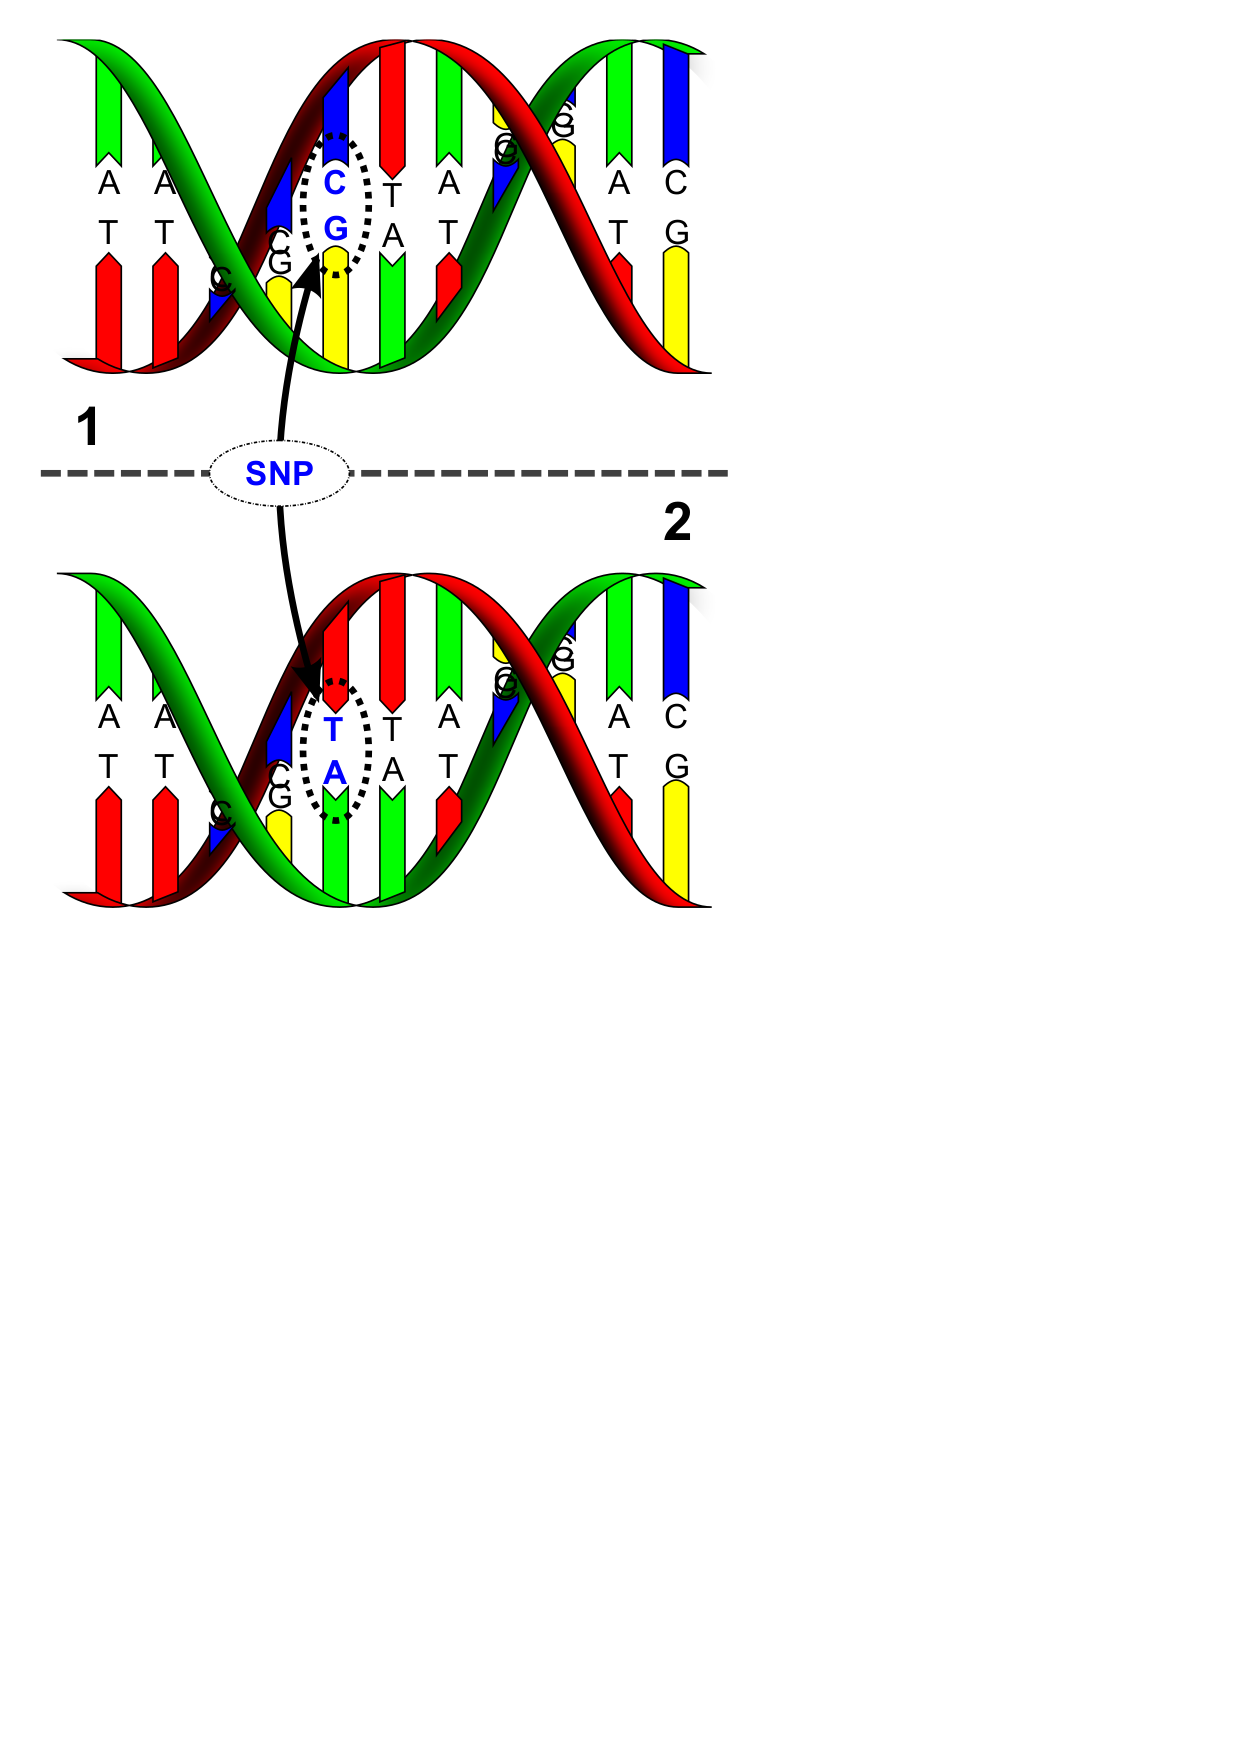
\includegraphics[height=4cm]{SNP}   
    \caption{SNP (wikipedia)}
  \end{figure}
\end{multicols}

\end{frame}

\begin{frame}
  \frametitle{Summarize 500,000 variables with 2 features}

  \begin{figure}
    \centering
      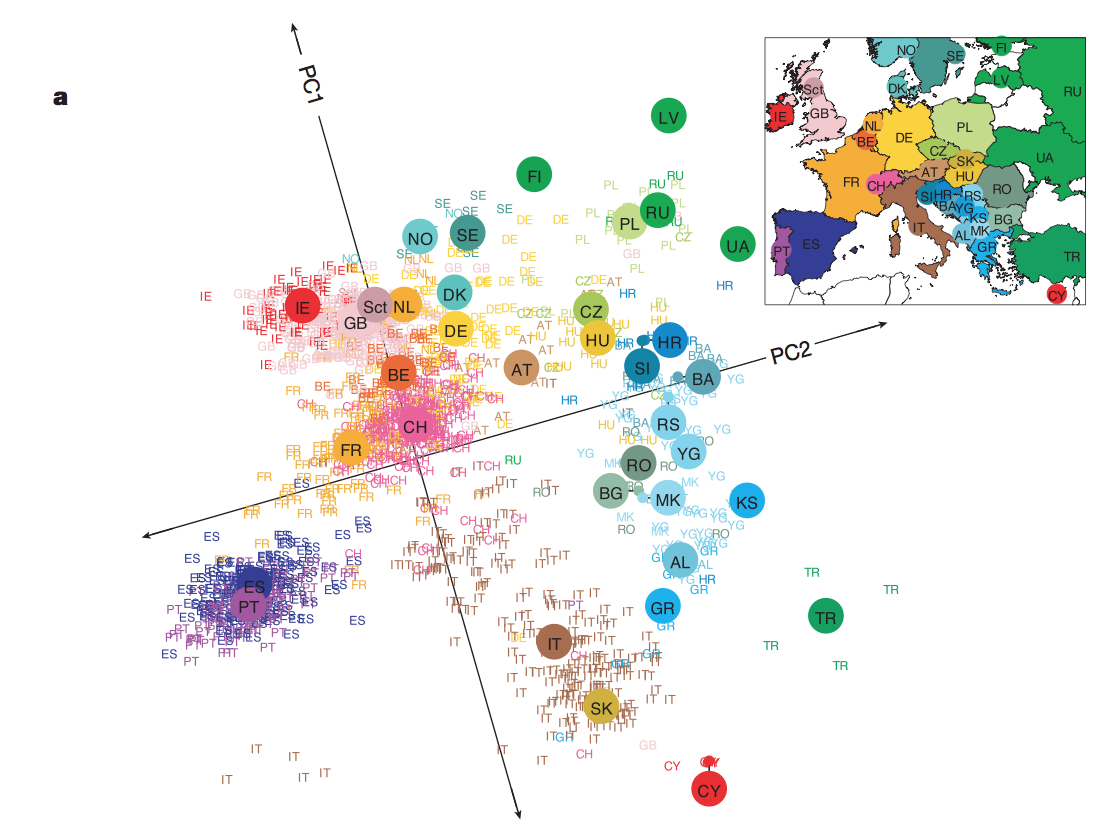
\includegraphics[height=5.5cm]{geneMirrorGeography}
    \caption{Dimension reduction + labels {\tiny source: Nature "Gene  Mirror Geography Within  Europe", 2008}}
  \end{figure}

  In the original messy $3,000 \times 500,000$ table, we may find
  \begin{itemize}
    \item an extremely strong structure between individuals (\alert{\bf "clustering"})
    \item a very simple subspace where it is obvious (\alert{\bf "dimension reduction"})
  \end{itemize}

\end{frame}

\begin{frame}[label=DimensionReduction]
  \frametitle{Dimension reduction: general goals}

  \paragraph{Main objective:} find a \alert{\bf low-dimensional representation} that captures the "essence" of (high-dimensional) data

  \vfill

  \begin{block}{Application in Machine Learning}
  \alert{Preprocessing, Regularization}
  \begin{itemize}
    \item Compression, denoising,  anomaly detection
    \item Reduce overfitting in supervised learning
  \end{itemize}
  \end{block}

\vfill

  \begin{block}{Application in Statistics/Data analysis}
    \alert{Better understanding of the data}
    \begin{itemize}
      \item descriptive/exploratory methods
      \item visualization (difficult to plot and interpret $> 3d$!)
    \end{itemize}
  \end{block}

\end{frame}
\end{frame}



\end{document}
